\documentclass[12pt]{article}

%Russian-specific packages
%--------------------------------------
\usepackage[T2A]{fontenc}
\usepackage[utf8]{inputenc}
\usepackage[english, russian]{babel}
%for search in russian
\usepackage{cmap}
% for markdown style quotes
\usepackage{csquotes}
%--------------------------------------

%Math-specific packages
%--------------------------------------
\usepackage{amsmath}
\usepackage{amssymb}

\def\d{ \mathrm{d} }
\def\norm{ \mathrm{n} }

\usepackage{amsthm}
\newtheorem{lemma}{Лемма}
\newtheorem{definition}{Определение}
\newtheorem*{remark}{Замечание}

%Format-specific packages
%--------------------------------------
\usepackage[left=2cm,
            right=2cm,
            top=1cm,
            bottom=2cm,
            bindingoffset=0cm]{geometry}

%Graphics packages
%--------------------------------------
\usepackage{graphicx}
\usepackage{wrapfig}

\graphicspath{ { ./tex/ } }

\includeonly{
  tex/title
  , tex/introduction
}

\usepackage{tikz}
\usetikzlibrary{
  shapes.geometric
  , intersections
  , calc
  % for angles
  , angles
  , quotes
  , babel
  % ------
 , external
 , arrows.meta
 , patterns
}
\tikzexternalize[prefix=tex/]

\begin{document}

\begin{titlepage}
  \begin{center}
    \large{Федеральное государственное бюджетное образовательное\\
      учреждение высшего образования\\}

    Московский государственный университет\\
    имени М. В. Ломоносова\\

    \vspace{0.25 cm}

    \normalsize{Механико-математический факультет\\}
    \vspace{0.5 cm}
    Кафедра вычислительной математики\\
  \end{center}

  \vspace{3cm}

  \begin{center}
    \LARGE{Курсовая работа}\\

    \vspace{0.5 cm}

    \normalsize{}
    \textbf{Тема:} \textit{Введение в Photometric Stereo.}
  \end{center}

  \vspace{3 cm}

  \begin{flushright}
    \textbf{Выполнил:}\\
    студент 4 курса
    431 группы\\

    \textit{Шерстобитов Андрей Сергеевич}\\

    \vspace{1 cm}

    \textbf{Научный руководитель:}\\

    \textit{Валединский Владимир Дмитриевич}
  \end{flushright}

  \vspace{\fill}
  \normalsize{}
  \begin{center}
    Москва\\2022
  \end{center}

  \thispagestyle{empty}
\end{titlepage}


\newpage
\tableofcontents

\newpage

\section{Вступление}

Photometric stereo — метод в компьютерном зрении для определения
нормалей поверхности объектов путем наблюдения за этим объектом
при различных условиях освещения. Он основан на том факте,
что количество света, отражаемого поверхностью, зависит от ориентации
поверхности относительно источника света и наблюдателя.

\begin{figure}[h]
  \centering
  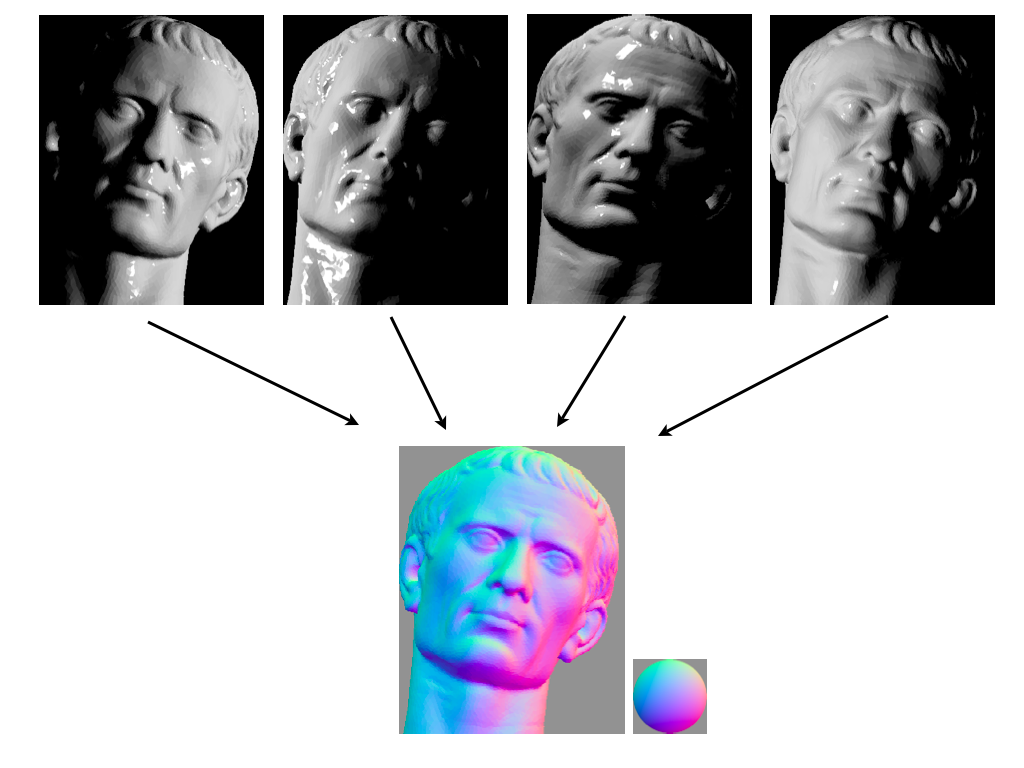
\includegraphics[scale=0.3]{tex/example.png}
\end{figure}

При использовании этого метода путем измерения количества света,
отраженного в камеру, пространство возможных ориентаций поверхности может
быть ограничено. Если объект наблюдается под достаточным количеством источников
света с разных углов, то ориентация поверхности может быть ограничена
до одной ориентации или даже получиться больше, чем необходимо.

Метод был впервые предложен в 1980 году Уодхэмом. Особый случай,
когда данные представлены одним изображением, известен как "shape from shading",
и был анализирован Б. К. П. Хорном в 1989 году. Расширенные методы фотометрического
стерео были разработаны для учета проецируемых теней и других
неоднородных условий освещения.

Однако, этот метод требует тщательного планирования и контроля эксперимента,
чтобы получить необходимое количество данных, и считается,
что он неэффективен для объектов с неоднородной поверхностью
и большим числом полостей. Тем не менее, photometric stereo все еще остается
важной технологией в области компьютерного зрения, особенно для задач
реконструкции трехмерных объектов.


\newpage

\section{Радиометрия}
\subsection{Телесный угол}

Познакомимся с понятием \textit{телесного угла}, разберемся как и в чем происходит измерение этой величины. Именно с него будет начинаться наше погружение
в Photometric stereo.

\begin{wrapfigure}[14]{r}{0.4\textwidth}
  \begin{center}
    \begin{tikzpicture}[scale=0.9,every node/.style={scale=0.9}]
      \draw (0,0) circle (2cm);
      \coordinate [label=below:$O$] (O) at (0,0);
      \draw [dashed] (0,0) -- node[above]{$R$} (-2,0);
      \draw (-2,0) arc (180:360:2 and 0.6);
      \draw [dashed] (2,0) arc (0:180:2 and 0.6);

      \node [ellipse,
        draw=black,
        fill=cyan!10,
        minimum width = 0.6cm,
        minimum height = 0.4cm,
        rotate=125] (e) at (0.9,0.9) {};
      \draw [dashed] (O) -- (e.east);
      \draw [dashed] (O) -- (e.west);

      \node [ellipse,
        draw=black,
        fill=cyan!20,
        minimum width = 1.8cm,
        minimum height = 1.2cm,
        rotate=125] (E) at (2.70,2.70) {};
      \draw (e.east) -- (E.east);
      \draw (e.west) -- (E.west);
      \coordinate [label=center:$\Sigma$] (S) at (E.center);

    \end{tikzpicture}
    \caption{Телесный угол}
  \end{center}
\end{wrapfigure}

Поставим наблюдателя в центр сферы $O$ радиуса $R$. Обозначим $\Sigma$ наблюдаемую
из точки $O$ поверхность. Площадь сферы покрываемую объектом обозначим $S$. Тогда величиной телесного угла
является следующее отношение:
$$\omega=\frac{S}{R^2}$$
Точка $O$ называется вершиной (apex) телесного угла.
\textbf{Телесный угол} - пучок лучей из $O$ до $\Sigma$.
Говорят, что наблюдатель \textit{стягивает} его телесный угол в вершине.

Единица измерения в системе  СИ - стерадиан (ср, sr), равный телесному углу,
вырезающему из сферы радиуса $R$ поверхность с площадью $R^2$.

\begin{remark}
  Площадь поверхности сферы = $4\pi R^2$, тогда полный телесный угол равен
  $$\omega=\frac{4\pi R^2}{R^2}=4\pi$$
\end{remark}

\begin{remark}
  Для кругового конуса с углом раствора $\theta$ телесный угол при его вершине
  равен $$\omega=\frac{2\pi R^2(1-\cos\theta)}{R^2}=2\pi(1-\cos\theta)$$
\end{remark}

\begin{wrapfigure}[10]{r}{0.35\textwidth}
  \begin{center}
    \begin{tikzpicture}[scale=0.75]
      \coordinate (O) at (0,0);
      \node [circle,
        name path=U,
        draw=black,
        minimum size=3cm] (U) at (O) {};
      \node [circle,
        draw=black,
        label=left:$S_0$] (S0) at (O) {};

      \coordinate (dAl) at (1,-7);
      \coordinate (dAr) at (3,-7);
      \coordinate (dAm) at ($(dAl)!0.5!(dAr)$);
      \coordinate (n) at (2,-6);
      \draw (dAl) -- (dAr);

      \draw [name path=O--dAl,dashed] (O) -- node [left] {$r$} (dAl);
      \draw [name path=O--dAr,dashed] (O) -- (dAr);
      \draw (O) -- (dAm) node [below] {$\d A$};

      \begin{scope}
        \path [name intersections={of=O--dAl and U,by=C}];
        \path [name intersections={of=O--dAr and U,by=D}];
        \draw [line width=1mm] (C) -- (D) node [right] {$\d A_0$};
      \end{scope}

      \draw [->, line width=0.5mm] (dAm) -- (n) node [right] {$\norm$};
      \pic [draw, angle radius=6mm,"$\theta$",left] {angle=n--dAm--O};
    \end{tikzpicture}
    \caption{Стянутый объектом $S_0$ телесный угол}
    \label{subtended}
  \end{center}
\end{wrapfigure}

Чаще всего бывает, что изучаемая поверхность находится под углом $\theta$
к наблюдателю. На рис. \eqref{subtended} $\norm$ это нормаль к
изучаемой поверхности $\d A$, $S_0$ - центр единичной окружности.
Расстояние между $S_0$ и $\d A$ обозначим $r$. Заметим, что угол между
нормалью плоскости $\norm$ и направлением взгляда наблюдателя обозначим $\theta$.
$\d A_0$ является проекцией $\d A$ на единичную сферу, тогда телесный угол имеет величину:
$$\d \omega = \frac{\d A\cos\theta}{r^2}$$

\newpage

\subsection{Сила света (Intensity)}

Простыми словами фотометрия - наука об измерении света с точки
зрения его яркости, воспринимаемой человеческим глазом.
Сразу можно задать вопрос: как и в чем измеряется
свет? Попытаемся формализировать ответы на эти вопросы.

Современное определение единицы силы света было зафиксировано в 1979 г.
XVI Генеральной конференцией по мерам и весам. Международной системе единиц (СИ)
имеет следующее описание:

\begin{displayquote}
  Сила света в заданном направлении источника, испускающего
  монохроматическое излучение частотой 540$\cdot$1012 Гц, энергетическая сила света
  которого в этом направлении составляет 1/683 Вт/ср.
\end{displayquote}

Единица силы света имеет общеприниятое название -- кандела (кд, cd).
Сила света имеет обозначение $I$.

Для силы света оказался верен закон обратных квадратов: значение силы света в
данной точке пространства обратно пропорицонально квадрату расстояния от источника света.
То есть имея два источника света с соотвествующими силами $I_1$ и $I_2$, расположенные
соответственно на расстояних $r_1$ и $r_2$ верно следующее равенство:

\begin{equation} \label{inverse_law}
  \frac{I_1}{I_2} = \frac{r_2^2}{r_1^2}
\end{equation}

\subsection{Поток (Flux)}

Рассмотрим некоторый источник света $S_0$ в некотором пространстве.
Излучаемый свет можно представить как совокупность телесных углов $\omega$ с вершиной
в источнике $S_0$. Пусть источник света имеет силу $I$.

\begin{figure}[h]
  \begin{center}
    \begin{tikzpicture}[
        declare function={lin(\t) = \t / 1.5;}
      ]
      \newcommand\connectEllipces[3]{
        \path [name intersections={of=S0--omega_east and #1,by=A}];
        \path [name intersections={of=S0--omega_west and #1,by=B}];
        \draw
        (#2) -- (A)
        (#3) -- (B);
      };

      \def \R {115};
      \tikzstyle{ellipse template}=[ellipse,draw=black,minimum width=1cm,minimum height=0.5cm,rotate=\R];

      \coordinate [label=left:$S_0$] (S0) at (0, 0);

      \def \OmegaScale {1};
      \path let \n1={8} in node [ellipse template
          , fill=gray
          , opacity=0.3
          , scale=\OmegaScale
          , name path=omega
        ] (omega) at (\n1,{ lin(\n1) }){};
      \node at (omega.center) {$\omega$};
      \coordinate (S0_omega_west_vector) at ($ (omega.west) - (S0) $);

      \draw [name path=S0--omega_east,dashed] (S0) -- (omega.east);
      \draw [name path=S0--omega_west,dashed] (S0) -- (omega.west);

      \path let \n1={2.4} in node [ellipse template
          , scale=1.5
          , name path=e] (e) at (\n1,{ lin(\n1) }) {};

      \draw [->] (S0) -- node [left] {$r_1$} (e.north east);
      \connectEllipces{e}{S0}{S0};

      \path [name path=e_vert] (e.west) -- (e.east);
      \path [name intersections={of=S0--omega_east and e_vert,by=e_omega_east}];
      \path [name intersections={of=S0--omega_west and e_vert,by=e_omega_west}];
      \path let
      \n1 = {2.4},
      \p2 = (S0_omega_west_vector),
      \p3 = ($ (e_omega_west) - (S0) $),
      \n4 = { veclen(\x3,\y3) / veclen(\x2,\y2) }
      in node [ellipse template
          , scale=\OmegaScale * \n4
          , name path=e_omega
        ] (e_omega) at (\n1,{ lin(\n1) }) {};
      \node [below] at (e_omega_west) {$\sigma_1$};

      \path let \n1={3.6} in node [ellipse template
          , scale=2.5
          , name path=E] (E) at (\n1,{ lin(\n1) }) {};

      \draw [->] (S0) -- node [below] {$r_2$} (E.north west);
      \connectEllipces{E}{e_omega_east}{e_omega_west};

      \path [name path=E_vert] (E.west) -- (E.east);
      \path [name intersections={of=S0--omega_east and E_vert,by=E_omega_east}];
      \path [name intersections={of=S0--omega_west and E_vert,by=E_omega_west}];
      \path let
      \n1 = {3.6},
      \p2 = (S0_omega_west_vector),
      \p3 = ($ (E_omega_west) - (S0) $),
      \n4 = { veclen(\x3,\y3) / veclen(\x2,\y2) }
      in node [ellipse template
          , scale=\OmegaScale * \n4
          , name path=E_omega
        ] (E_omega) at (\n1,{ lin(\n1) }) {};
      \node [below] at (E_omega_west) {$\sigma_2$};

      \path let \n1={5.6} in node [ellipse template
          , scale=4
          , name path=EE] (EE) at (\n1,{ lin(\n1) }) {};

      \draw [->] (S0) -- node [below] {$r_3$} (EE.west);
      \connectEllipces{EE}{E_omega_east}{E_omega_west};

      \path [name path=EE_vert] (EE.west) -- (EE.east);
      \path [name intersections={of=S0--omega_east and EE_vert,by=EE_omega_east}];
      \path [name intersections={of=S0--omega_west and EE_vert,by=EE_omega_west}];
      \path let
      \n1 = {5.6},
      \p2 = (S0_omega_west_vector),
      \p3 = ($ (EE_omega_west) - (S0) $),
      \n4 = { veclen(\x3,\y3) / veclen(\x2,\y2) }
      in node [ellipse template
          , scale=\OmegaScale * \n4
          , name path=EE_omega
        ] (EE_omega) at (\n1,{ lin(\n1) }) {};
      \node [below] at (EE_omega_west) {$\sigma_3$};

      \draw
      (EE_omega_east) -- (omega.east)
      (EE_omega_west) -- (omega.west);

    \end{tikzpicture}
    \caption{Световой поток источника $S_0$ внутри угла $\omega$}
  \end{center}
\end{figure}

Произвольными радиусами $r_1$, $r_2$, $r_3$ построим сферы с центром в вершине
телесного угла $S_0$ и обозначим выделенные телесным углом площади на сферах соответсвенно
$\sigma_1$, $\sigma_2$, $\sigma_3$. За единицу времени на эти площади упадет одна и та
же энергия: $\frac{I}{r_1^2}\sigma_1$, $\frac{I}{r_2^2}\sigma_2$, $\frac{I}{r_3^2}\sigma_3$.
Обратим внимание, что $\frac{\sigma_1}{r_1^2}=\frac{\sigma_2}{r_2^2}=\frac{\sigma_3}{r_3^2}=\omega$.
Таким образом, \textbf{поток} - физическая величина пропорциональная световой мощности,
переносимой пучком лучей, распространяющимися внутри телесного угла $\omega$.
\[\Phi:=I\omega\]
Световой поток, выходящий из телесного угла 1ср, с силой света 1кд называется \textit{люмен} (лм, lm).

Обратим внимание, что в качестве источника света здесь рассматривается вершина телесного угла, то есть
точка в пространстве, но в жизни же источники света не только не могут быть точкой, но и могут
достигать весьма больших размеров. Всегда стоит помнить, что если речь идет об источнике света
как о точке, то подразумевается, что расстояние между освещаемым объектом во много раз
превышает размер источника и, в следствие различные лучи источника попадают в достаточно малый телесный угол.

\subsection{Освещенность (Irradiance)}

Зафиксируем точечный источник света $S_0$ с силой света $I$ на расстоянии $r$ от поверхности площадью $\sigma$.
\begin{figure}[h]
  \begin{center}
    \begin{tikzpicture}
      \node [circle,
        draw=black,
        scale=0.4,
        label=left:$S_0$] (S0) at (0,0) {};
      \coordinate (S0) at (S0);

      \coordinate (Au) at (7,1);
      \coordinate (Al) at (7,-1);
      \draw (Au) -- node[right]{$\sigma$} (Al);
      \draw (Au) -- (S0) -- (Al);
      \draw [-{Stealth[scale=2]}] (S0) -- node[above]{$r$} ($(Au)!0.5!(Al)$);
    \end{tikzpicture}
    \caption{Лучи $S_0$, падающие по нормали к поверхности}
  \end{center}
\end{figure}

Величина
\begin{equation}\label{irradiance}
  E:=\frac{I}{r^2}
\end{equation}

является мерой освещения, получающегося на поверхности при падении лучей под прямым углом.

За единицу освещенности принимается такая освещенность, которую создает
источник силой света в 1 кд, освещающий по нормали поверхность,
отстояющую от него на расстояние 1 м. Единица освещенности — люкс (лк, lx).

Проводя аналогии с физическими величинами, можно сравнить освещенность с плотностью потока.
Действительно, домножив числитель и знаменатель \eqref{irradiance} на бесконечно малый телесный
угол $\d\omega$, получим следующее

\[E=\frac{I\d\omega}{r^2\d\omega}=\frac{\d\Phi}{\d\sigma}\]

\begin{figure}[h]
  \begin{center}
    \begin{tikzpicture}
      \node [circle,
        draw=black,
        scale=0.4,
        label=left:$S_0$] (S0) at (0,0) {};
      \coordinate (S0) at (S0);

      \coordinate (Au) at (7,1);
      \coordinate (Al) at (9,-1);
      \coordinate (Am) at ($(Au)!0.5!(Al)$);
      \path let \p1=($ (Au) - (Al) $) in node (N) at ([shift={(-\y1,\x1)}]Am){$N$};
      \draw (Au) -- node[right,scale=1.5]{$\frac{\sigma}{\cos\phi}$} (Al);
      \draw (Au) -- (S0) -- (Al);
      \draw [-{Stealth[scale=2]}] (S0) -- node[above]{$r$} (Am);
      \draw [-{Stealth[scale=2]}] (Am) -- (N);
      \pic [draw, angle radius=20mm,"$\phi$",left] {angle=S0--Am--N};
    \end{tikzpicture}
    \caption{Лучи $S_0$, падающие под углом $\phi$}
    \label{irradiance_under_angle}
  \end{center}
\end{figure}

В случае, когда лучи источника падают под углом $\phi$ к нормали на Рис. \eqref{irradiance_under_angle}, сила светового
потока распределяется по увеличнной площади, в следствие чего освещенность поверхности
оказывается меньше:

\begin{equation}
  E=\frac{\d\Phi}{\d\sigma/\cos\phi}=\frac{I}{r^2}\cos\phi
\end{equation}

\subsection{Энергетическая яркость (Radiance)}

На рисунке \eqref{radiance_pic} в качестве источника рассматривается бесконечно
малая площадь поверхности $\d\sigma_1$, в качестве получателя рассматривается бесконечно
малая площадь поверхности $\d\sigma_2$, расстояние между ними конечно и равно $r$.
Пусть нормаль $\norm_1$ поверхности $\d\sigma_1$ образует с пучком света угол $\phi_1$,
нормаль $\norm_2$ соответсвенно $\phi_2$.

\begin{figure}[h]
  \begin{center}
    \begin{tikzpicture}
      \tikzstyle{trapezium template}=[trapezium, draw, minimum width=3cm, trapezium left angle=120, trapezium right angle=60, scale=0.5]

      \node [trapezium template, rotate=30] (L) at (0, 0){};
      \node [trapezium template, rotate=-30] (R) at (7, 0){};
      \node [draw=black,circle,scale=0.3] (Lc) at (L.center){};
      \node [draw=black,circle,scale=0.3] (Rc) at (R.center){};

      \draw [-{Stealth[scale=2]}] (Lc) -- node[above]{$r$} (Rc);

      \path let \p1=($ (L.north) - (L.south) $) in node (LN) at ([shift={(1.5,1.5)}]Lc){$\norm_1$};
      \draw [->] (Lc) -- (LN);
      \pic [draw, angle radius=12mm,"$\phi_1$"] {angle=Rc--Lc--LN};

      \path let \p1=($ (R.north) - (R.south) $) in node (RN) at ([shift={(-1.5,-1.5)}]Rc){$\norm_2$};
      \draw [->] (Rc) -- (RN);
      \pic [draw, angle radius=12mm,"$\phi_2$"] {angle=Lc--Rc--RN};

    \end{tikzpicture}
    \caption{Световой поток пластинки $\d\sigma_1$ на $\d\sigma_2$}
    \label{radiance_pic}
  \end{center}
\end{figure}

По определению световой поток должен быть пропорционален площадям
проекций каждой из площадок $\d\sigma_1$ и $\d\sigma_2$ на плоскость,
перпендикулярную направлению падающего пучка, и обратно пропорционален квадрату
расстояния между ними. Его можно представить в следующей форме

\begin{equation}\label{radiance::origin}
  \d^2\Phi=L\frac{\d\sigma_1\cos\phi_1\d\sigma_2\cos\phi_2}{r^2}
\end{equation}

Коэффициент пропорциональности $L$
называется \textbf{яркостью} излучающего элемента $\d\sigma_1$ в направлении
к освещаемому элементу $\d\sigma_2$.

Рассмотрим выражение \eqref{radiance::origin} иначе. Возьмем за источник $\d\sigma_1$ с силой $\d I$,
тогда световой поток, падающий на пластинку $\d\sigma_2$, можно представить следующим образом:
\begin{equation}\label{radiance::flux_on_receiver}
  \d^2\Phi=\d E_2\d\sigma_2=\frac{\d I}{r^2}\cos\phi_2\d\sigma_2
\end{equation}
Из \eqref{radiance::origin} и \eqref{radiance::flux_on_receiver} следует
\begin{equation}\label{radiance::result}
  L = \frac{\d I}{\d\sigma_1\cos\phi_1}
\end{equation}

Выражение \eqref{radiance::result} определяет \textit{яркость поверхности в заданной точке
  и в заданном направлении}. Единица яркости -- кандела на квадратный метр (кд/м$^2$).


\newpage

\section{Поверхности}

\subsection{Двулучевая функция отражательной способности (BRDF)}

Очевидно, что яркость точки на поверхности как-то зависит от материала поверхности,
на которую падает свет. Иначе говоря, яркость зависит от так называемых отражательных
способностей поверхности. На Рис. \eqref{brdf} компьютером отрисованы различные сферы.
В данном примере и камера и источник света находятся относительно далеко от сфер.
Причина, по которой мы видим их различными -- их материал, или различные отражательные способности.

\begin{figure}[h]
  \centering
  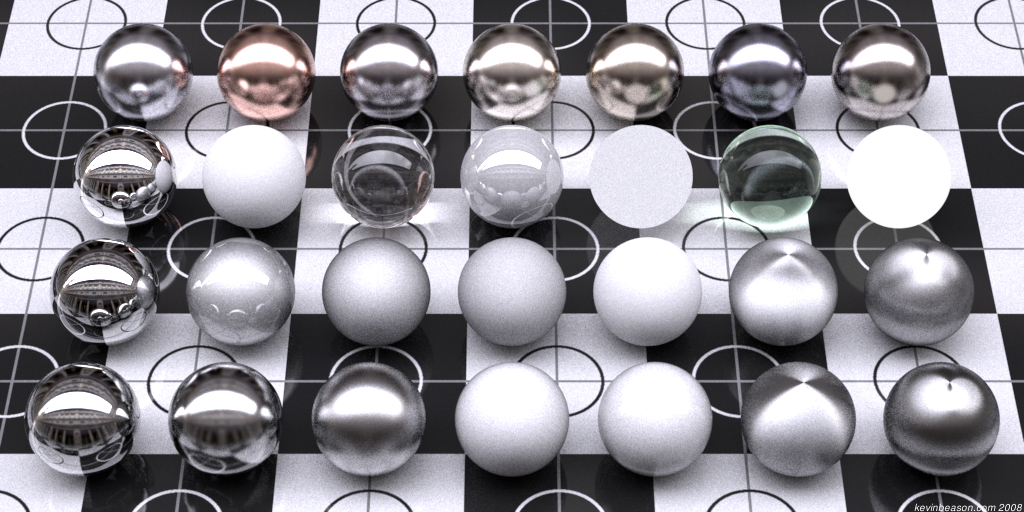
\includegraphics[scale=0.3]{tex/brdf.png}
  \caption{Пример разных отражательных способностей}
  \label{brdf}
\end{figure}

Возникает идея формализировать представление отражательных способностей любого материала,
с чем нам поможет двулучевая функция отражательной способности или ДФОС.

Для определения нам важны направления: направление света, падающего на предмет, и направление
отраженного и полученного света. Двулучевая функция, потому что речь будет идти про два луча.

\begin{figure}[h]
  \begin{center}
    \begin{tikzpicture}
      \def\SndrAngle {225};
      \def\SndrColor {yellow};
      \node [draw,
        fill=\SndrColor,
        rectangle,
        minimum width=1cm,
        minimum height=0.5cm,
        rotate=\SndrAngle,
      ] (SndrRect) at (-5, 4){};
      \filldraw[fill=\SndrColor] let
      \p1=($ (SndrRect.north west) - (SndrRect.north east) $),
      \n2={0.3}
      in
      ($ (SndrRect.north east)!.5!(SndrRect.north) $) coordinate (SndrA) --
      ($ (SndrRect.north)!.5!(SndrRect.north west) $) coordinate (SndrB) --
      ([shift={(\y1*\n2,-\x1*\n2)}]SndrRect.north west) coordinate (SndrC) --
      ([shift={(\y1*\n2,-\x1*\n2)}]SndrRect.north east) coordinate (SndrD) -- cycle
      ;
      \node[left,text width=2.5cm] at (SndrRect.south east) {Источник (Прожектор)};

      \def\RcvrColor {gray};
      \node [draw,
        fill=\RcvrColor,
        rectangle,
        minimum width=1cm,
        minimum height=0.5cm,
        rotate=360-\SndrAngle,
      ] (RcvrRect) at (5, 4){};
      \filldraw[fill=\RcvrColor] let
      \p1=($ (RcvrRect.north west) - (RcvrRect.north east) $),
      \n2={0.3}
      in
      ($ (RcvrRect.north east)!.5!(RcvrRect.north) $) coordinate (RcvrA)
      -- ($ (RcvrRect.north)!.5!(RcvrRect.north west) $) coordinate (RcvrB)
      -- ([shift={(\y1*\n2,-\x1*\n2)}]RcvrRect.north west) coordinate (RcvrC)
      -- ([shift={(\y1*\n2,-\x1*\n2)}]RcvrRect.north east) coordinate (RcvrD)
      -- cycle
      ;
      \node[right,text width=2.5cm] at (RcvrRect.south west) {Получатель (Камера)};

      \node [draw,
        trapezium,
        shade,
        minimum width=3cm,
        trapezium left angle=120,
        trapezium right angle=60] (Srfc) at (0, 0){};

      \draw[-Stealth, thick]
      (Srfc.center) coordinate (beginN)
      -- ([shift={(0,1.5)}]Srfc.center) coordinate (endN) node[above]{$\norm$};

      \draw[-Stealth,color=\SndrColor,line width=0.5mm]
      ($ (SndrC)!.5!(SndrD) $) coordinate (beginSnd)
      --node[left,color=black]{$(\theta_i,\phi_i)$} (Srfc.center) coordinate (endSnd);

      \draw[-Stealth,color=\RcvrColor,line width=0.5mm]
      (Srfc.center) coordinate (beginRcv)
      --node[right,color=black]{$(\theta_r,\phi_r)$} ($ (RcvrC)!.5!(RcvrD) $) coordinate (endRcv);

    \end{tikzpicture}
    \caption{Отражение поверхности}
    \label{surface_reflection}
  \end{center}
\end{figure}

Таким образом, чтобы представить свойства отражения любого материала,
мы хотим иметь возможность описать его свойства как с точки зрения
направления освещения, так и с точки зрения направления взгляда или направления отражения.

Выражая направление источника в полярных координатах через углы $(\theta_i,\phi_i)$ и
направление отраженного света через $(\theta_r,\phi_r)$, мы можем следующее
\begin{enumerate}
  \item Освещенность поверхности зависит от углов $(\theta_i,\phi_i)$, то есть $E:=E(\theta_i,\phi_i)$.
  \item Яркость поверхности зависит от углов $(\theta_r,\phi_r)$, то есть $L:=L(\theta_r,\phi_r)$.
\end{enumerate}

И теперь мы можем описать отражательную способность как двулучевую функцию отражательной
способноси:
\begin{equation}
  \rho(\theta_i,\phi_i,\theta_r,\phi_r)=\frac{L(\theta_r,\phi_r)}{E(\theta_i,\phi_i)}
\end{equation}

Измеряется в ср$^{-1}$, где стерадиан (ср) - единица измерения телесного угла. Перечислим некоторые свойства ДФОС:
\begin{enumerate}
  \item Неотрицательность: $\rho(\theta_i,\phi_i,\theta_r,\phi_r)>0$. Следует из того, что и
        яркость, и освещенность неотрицательны, значит и их отношение.
  \item Удовлетворяет равенству Гельмгольца: $\rho(\theta_i,\phi_i,\theta_r,\phi_r)=\rho(\theta_r,\phi_r,\theta_i,\phi_i)$.
        Это нам говорит о том, что поменяв местами прожектор и камеру, мы получим то же самое значение ДФОС.
\end{enumerate}

Существуют множество поверхностей, которые отражают одинаковое количество света
вне зависимости от вращения этой поверхности вокруг ее нормали. Такие
поверхности называют \textit{изотропными}, в обратном случае \textit{анизотропными}.
Когда говорят об изотропных поверхностях ДФОС определяют как функцию принимающую три
аргумента вместо четырех: $\rho(\theta_i,\theta_r,\phi)$.

\subsection{Механизмы, порождающие отражение}

Давайте поговорим об основных механизмах, порождающие отражение света.

\begin{figure}[h]
  \centering
  \begin{minipage}{.5\textwidth}
    \centering
    \begin{tikzpicture}
      \node [draw,
        rectangle,
        minimum width=6cm,
        minimum height=0.5cm,
      ] (obj) at (0, -1){};

      \draw[-Stealth, thick, black] (-3,3) coordinate (src) --node[above, midway, sloped]{Источник} ($ (obj.north east)!.5!(obj.north west) $) coordinate (middle);
      \draw[-Stealth, thick, blue] (middle) --node[above, midway, sloped]{Зеркальное отражение} (3,3) coordinate;
    \end{tikzpicture}
  \end{minipage}%
  \begin{minipage}{.5\textwidth}
    \centering
    \begin{tikzpicture}
      \node [draw,
        rectangle,
        pattern=bricks,
        minimum width=6cm,
        minimum height=1cm,
      ] (obj) at (0, -1){};
      \draw[-Stealth, thick, black] (-3,3) coordinate (src) --node[above, midway, sloped]{Источник} ($ (obj.north east)!.5!(obj.north west) $) coordinate (middle);
      \node [circle,
        inner sep=0pt,
        outer sep=0pt,
        minimum size=3cm] (C1) at (0,1) {};
      \draw[-Stealth, thick, red] (middle) -- (C1.north) coordinate node[right]{Диффузное отражение};
      \draw[-Stealth, thick, red] (middle) -- (C1.north west) coordinate;
      \draw[-Stealth, thick, red] (middle) -- (C1.north east) coordinate;
      \draw[-Stealth, thick, red] (middle) -- (C1.west) coordinate;
      \draw[-Stealth, thick, red] (middle) -- (C1.east) coordinate;
      \draw[-Stealth, thick, red] (middle) -- (C1.south west) coordinate;
      \draw[-Stealth, thick, red] (middle) -- (C1.south east) coordinate;
      \node [circle,
        inner sep=0pt,
        outer sep=0pt,
        rotate=22.5,
        minimum size=3cm] (C2) at (0,1) {};
      \draw[-Stealth, thick, red] (middle) -- (C2.north) coordinate;
      \draw[-Stealth, thick, red] (middle) -- (C2.north west) coordinate;
      \draw[-Stealth, thick, red] (middle) -- (C2.north east) coordinate;
      \draw[-Stealth, thick, red] (middle) -- (C2.west) coordinate;
      \draw[-Stealth, thick, red] (middle) -- (C2.east) coordinate;
      \draw[-Stealth, thick, red] (middle) -- (C2.south) coordinate;
      \draw[-Stealth, thick, red] (middle) -- (C2.south west) coordinate;
      \draw[-Stealth, thick, red] (middle) -- (C2.south east) coordinate;
    \end{tikzpicture}
  \end{minipage}
  \caption{Диффузное и зеркальное отражение}
  \label{reflect}
\end{figure}

Рассмотрим рис. \eqref{reflect}. Различают три механизма:
\begin{itemize}
  \item Первый - отражательная способность поверхности. Свет падает на поверхность
        и отражение происходит на самой плоскости. Такое отражение света называется
        \textit{зеркальны м} отражением. Оно придает поверхностям глянцевый или блестящий
        вид и свойственно гладким однородным материалам (зеркалам, стеклу, полированным металлам).
  \item Второй случай возникает, когда часть света проходит сквозь поверхность
        и проникает внутрь материала. Обычно вещества неоднородны и содержат различные
        частицы с разными показателями преломления. В результате попадающий внутрь свет
        преломляется и отражается несколько раз, отскакивает внутри случайным образом.
        Это происходит на небольшой глубине под поверхностью, поэтому частицы света
        проникают обратно и рассеиваются во многих направлениях.
        Это явление называется \textit{диффузным}. Из-за неоднородности среды
        объекты обладают матовостью.
  \item При анализе яркости точки изображения надо учитывать, что это результат отражения света из окружающей среды, который имеет составляющие
        диффузного и поверхностного отражения. Чаще всего встречается \textit{гибридное} отражение — комбинация этих двух механизмов.
\end{itemize}

\subsection{Модели отражения}

Рассмотрим широко используемые модели отражения.

\subsubsection{Светорассеивающая поверхность, закон Ламберта}

Большинство предметов, с которыми нам чаще всего приходится работать в жизни
(бумага, песок, камень, мел), рассеивают падающий на них свет таким образом,
что их яркости в разных направлениях оказываются примерно одинаковыми.

В 1760 году немецкий ученый Ламберт сформулировал закон, согласно которому
\textit{яркости светорассеивающей поверхности во всех направлениях одинаковы}.
Хоть и установлено, что не существует предмета, который бы строго удовлетворял
закону Ламберта, этот закон часто используют в компьютерном зрении и
компьютерной графике, потому что несмотря на ее простоту она
позволяет достаточно точно описывать многие поверхности.

\begin{figure}[h]
  \centering
  \begin{tikzpicture}
    \draw [name path=arc] (0,0) arc (0:180:4cm and 4cm) -- cycle;
    \node [
      rectangle,
      name path=rec,
      minimum width=1cm,
      minimum height=0.2cm,
      pattern=north east lines] (rec) at (-4,-0.1){};
    \node [below] at (rec.south){$\sigma$};
    \path [name path=ll-rec] (-9,3.75) coordinate (ll) -- (rec.north) coordinate (m);
    \path [name path=lu-rec] (-8,4.25) coordinate (lu) -- (m);
    \path [name path=rl-rec] ( 1,3.75) coordinate (rl) -- (m);
    \path [name path=ru-rec] ( 0,4.25) coordinate (ru) -- (m);
    \path [name intersections={of=ll-rec and arc,by=A}];
    \path [name intersections={of=lu-rec and arc,by=B}];
    \path [name intersections={of=rl-rec and arc,by=C}];
    \path [name intersections={of=ru-rec and arc,by=D}];
    \fill [pink, opacity=0.3] (A) -- (C) -- (D) -- (B);

    \draw (A) -- (m) -- (C);
    \draw (B) -- (m) -- (D);
    \draw [dashed] (A) node [left] {$A$} -- (C) node [right] {$C$};
    \draw [dashed] (B) node [left] {$B$} -- (D) node [right] {$D$};
    \draw [->] let \p1 = (m) in (m) -- (\x1,4.2) coordinate (N) node[above]{$\norm$};
    \pic [<->, draw, angle radius=15mm,"$\phi$",angle eccentricity=1.2] {angle=D--m--N};
    \pic [<->, draw, angle radius=15mm,"$\d\phi$",angle eccentricity=1.2] {angle=C--m--D};
  \end{tikzpicture}
  \caption{Расчет светового потока, излучаемого поверхностью с постоянной яркостью}
  \label{lambert::pic}
\end{figure}

На Рис. \eqref{lambert::pic} рассматривается площадка площади $\sigma$,
яркость $L$ которой одинакова во всех направлениях.
Сила света в направлении к точке $D$: $I=L\sigma\cos\phi$.
Рассмотрим телесный угол $\d\omega$, заключенный между двумя конусами,
полученными вращениями прямых проведенных от середины
площадки до точек $C$ и $D$ вокруг нормали $\norm$. Посчитаем его значение:
$$\d\omega=2\pi(\cos\phi-\cos\phi\cos\d\phi+\sin\phi\sin\d\phi)\approx 2\pi\sin\phi\d\phi$$
Так как сила света внутри этого телесного угла постоянна, то световой поток, получаемый из площадки:
$$\d\Phi=I\d\omega=2\pi L\sigma\cos\phi\sin\phi\d\phi$$
Тогда чтобы получить световой поток, излучаемой площадкой, для всей полусферы:
\begin{equation}\label{lambert::eq}
  \Phi=2\pi L\sigma\int_0^{\frac{\pi}{2}} \cos\phi\sin\phi\d\phi=\pi L\sigma\sin^2\phi\vert_0^\frac{\pi}{2}=\pi L\sigma
\end{equation}
Если взять в качестве площадки объект, который отражает весь падающий на него поток
и рассеивает его так, что яркость во все стороны оказывается одинаковой (удовлетворяет свойствам
\textit{идеального рассеивателя}), то выражение \eqref{lambert::eq} можно
переписать следующим образом:
$$\frac{1}{\pi}=\frac{L\sigma}{\Phi}=\frac{L}{E}=\rho(\theta_i,\theta_r,\phi)$$
Получается, что для светорассеивающей поверхности, удовлетворяющей закону Ламберта, ДФОС
является константой.

Поверхность любого тела не обладает свойствами идеального рассеивателя,
поэтому для того чтобы численно характеризовать изменение яркости
в разных направлениях используют \textit{коэффициент яркости} или \textit{альбедо}.
Принято обозначать греческой буквой $\beta$, $0\leq\beta\leq1$.
Тогда выражение ДФОС по фиксированному направлению для любого тела имеет вид:
\begin{equation}
  \rho(\theta_i,\phi_i,\theta_r,\phi_r)=\frac{\beta}{\pi}
\end{equation}

\subsubsection{Зеркальная поверхность}

Рассмотрим противоположную модель - модель для идеально зеркальной поверхности.
Все отражение происходит на поверхности, диффузное отражение отсутствует.
В этом случае вся энергия падающего света отражается в одном направлении.

\begin{figure}[h]
  \begin{center}
    \begin{tikzpicture}
      \def\SndrAngle {225};
      \def\SndrColor {yellow};
      \node [draw,
        fill=\SndrColor,
        rectangle,
        minimum width=1cm,
        minimum height=0.5cm,
        rotate=\SndrAngle,
      ] (SndrRect) at (-5, 4){};
      \filldraw[fill=\SndrColor] let
      \p1=($ (SndrRect.north west) - (SndrRect.north east) $),
      \n2={0.3}
      in
      ($ (SndrRect.north east)!.5!(SndrRect.north) $) coordinate (SndrA) --
      ($ (SndrRect.north)!.5!(SndrRect.north west) $) coordinate (SndrB) --
      ([shift={(\y1*\n2,-\x1*\n2)}]SndrRect.north west) coordinate (SndrC) --
      ([shift={(\y1*\n2,-\x1*\n2)}]SndrRect.north east) coordinate (SndrD) -- cycle
      ;

      \def\RcvrColor {gray};
      \node [draw,
        fill=\RcvrColor,
        rectangle,
        minimum width=1cm,
        minimum height=0.5cm,
        rotate=120,
      ] (RcvrRect) at (4.5, 2){};
      \filldraw[fill=\RcvrColor] let
      \p1=($ (RcvrRect.north west) - (RcvrRect.north east) $),
      \n2={0.3}
      in
      ($ (RcvrRect.north east)!.5!(RcvrRect.north) $) coordinate (RcvrA)
      -- ($ (RcvrRect.north)!.5!(RcvrRect.north west) $) coordinate (RcvrB)
      -- ([shift={(\y1*\n2,-\x1*\n2)}]RcvrRect.north west) coordinate (RcvrC)
      -- ([shift={(\y1*\n2,-\x1*\n2)}]RcvrRect.north east) coordinate (RcvrD)
      -- cycle
      ;

      \node [draw,
        trapezium,
        shade,
        minimum width=3cm,
        trapezium left angle=120,
        trapezium right angle=60] (Srfc) at (0, 0){};

      \draw[-Stealth, thick]
      (Srfc.center) coordinate (beginN)
      -- ([shift={(0,1.5)}]Srfc.center) coordinate (endN) node[above]{$\norm$};

      \draw[-Stealth,color=\SndrColor,line width=0.5mm]
      ($ (SndrC)!.5!(SndrD) $) coordinate (beginSnd)
      --node[left,color=black]{$(\theta_i,\phi_i)$} (Srfc.center) coordinate (endSnd);

      \draw[-Stealth, dashed, color=blue, line width=0.5mm]
      let \p1=(beginSnd) in
      (Srfc.center) --node[above, midway, sloped]{Зеркальное отражение} (-\x1,\y1);

      \draw[-Stealth,color=\RcvrColor,line width=0.5mm]
      (Srfc.center) coordinate (beginRcv)
      --node[right,color=black]{$(\theta_r,\phi_r)$} ($ (RcvrC)!.5!(RcvrD) $) coordinate (endRcv);

    \end{tikzpicture}
    \caption{Отражение зеркальной поверхности}
    \label{specular_surface}
  \end{center}
\end{figure}

ДФОС в случае идеального зеркала выглядит следующим образом:

\begin{equation}
  \rho(\theta_i,\phi_i,\theta_r,\phi_r)=\frac{\delta(\theta_i-\theta_r)\delta(\phi_i+\pi-\phi_r)}{\cos\theta_i\sin\theta_i}
\end{equation}

где $\delta(x)=\begin{cases}
    1, & x=0    \\
    0, & x\neq0
  \end{cases}$, то есть это обозначает, что наблюдатель видит свет только когда вектор наблюдения совпадает с вектором отражения.

В знаменателе произведение косинуса и синуса, коэффициент пропорциональности, обеспечивающий выполнение закона сохранения энергии: весь свет, отражаемый сферой независимо от направления, равен свету, падающему на поверхность.

\newpage

\section{Photometric stereo}

\subsection{Обзор}

% Photometric stereo -- способ восстановить трехмерную форму объекта
% используя 
So now with all that in place we are
ready to develop our first method
for recovering three-dimensional shape information from image
intensity values.
First, let's take a look at the factors
that affect image intensity.
Let's say you measure one intensity
in the image, what are the factors that
drive that intensity value?
So here you see a typical imaging set up.
You have a camera with a viewing direction v,
we'll assume that the viewing direction is aligned
with the z-axis of your coordinate frame,
and we have a single light source here.
We're going to assume for our purposes
here that you have a single point light
source, which is in the direction s,
s is a unit vector.
It has a certain brightness, it has a certain distance
from the surface itself.
And the point that we are looking
at has a surface orientation, which
is described by the normal vector, unit normal vector n.
So image intensity is a function of the source.
Once again, the source is given by its direction,
its radiant intensity, its distance,
and it is determined by the orientation of the surface, n,
which has a couple of parameters associated with it,
and last but not least, the reflectance properties
of the surface.
And that could have several parameters or a small number
of parameters depending on how complex
the bidirectional reflectance distribution function is.
So in this lecture, for developing photometric stereo,
we're going to assume that we know
the source or the illumination.
When we say that the source is known
we are going to assume that we know not only
its direction but its radiant intensity and distance as well.
You're also assuming that it's a point light source.
And those point light source is distant from the surface.
What does that mean?
It means that as you walk around on the surface,
you're going to be seeing the source in the same direction
if the source is distant.
And we're going to assume that we
know the reflectance properties of the surface,
that is we are in a structured environment
where we have access to information
such as the reflectance properties
and we can control the lighting and therefore
we know the source direction.
And of course we've measured an intensity value in the image.
So I is known, the source is known,
and the reflectance properties are known,
and what we seek to estimate is the surface
normal at each point on the surface.
So that is really what photometric stereo does.
Photometric stereo is a way of computing, estimating
the surface normal at each point on the surface given
its reflectance properties and given information
about the light sources.
And it turns out in order to solve this problem,
we need more than one image more than one light source
so photometric stereo uses multiple light sources,
captures multiple images, and then from this stack of images
it's able to compute the surface orientation at each point.
So first we're going to start off with what's
called the gradient space.
The gradient space gives you a convenient representation
for the orientation or surface normal at each point
in the surface.
And then with the gradient space in place,
we're going to talk about the concept of a reflectance map.
It's a representation.
The reflectance map gives you the mapping
between surface orientation or surface
gradient and the intensity that a point would produce.
So the reflectance map assumes that you know the reflectance properties
of the surface, you know everything
you need to know about the light source
and then given a surface orientation,
it tells you what the corresponding image
intensity would be.
So with that in place, we can develop photometric stereo.
And we see that if you're given one intensity value, which
is measured using a single light source,
there are an infinite number of surface normals or surface
gradients that would have produced the same intensity
value.
And so to resolve this ambiguity,
we use multiple light sources and then
we find that we can with a small number of light sources
typically, uniquely determine the surface
normal at each point on the surface.
Now, there are circumstances where
we can write an expression for the reflectance model
of the surface.
We know what we are dealing with, we
know that it has a simple form and we can express it
as an equation, the bidirectional reflectance
distribution function.
The Lambertian model is an example of that.
But there are many other scenarios
where that information is not easily available.
In other words, we know what we are dealing with,
the materials that we're dealing with,
but we don't know exactly what the BRDF of the material
is.
So in this case, we can develop what's
called a calibration-based approach, a data driven
approach.
That is let's assume that you're talking about painted objects.
We can take our paint and paint an object
of known shape with that same paint,
and then use that calibration object
to create a look up table that allows you to then take
image intensity values measured
on the real object, the object of interest,
and mapped them to surface orientations or surface
gradients.
So after you have applied photometric stereo, what
you end up with is the surface normal at each point
on the object.
And if the surface is continuous,
we can now integrate these surface normals
to recover the three-dimensional shape of the object.
So we look at an elegant approach
for integrating surface normal maps to obtain 3D shape.


\subsection{Градиент поверхности и нормаль}

Surface Gradient and Normal
Now let's take a look at an elegant, simple way
to represent surface orientation information,
and that is called the gradient space.
So let's assume that this is your surface right here,
z equal to f of xy.
At each xy, you know z, which is the depth of the surface.
And so we know that the surface gradient
is defined as the derivative of z with respect to x.
We take the negative of that, and we call that p.
We take the derivative of z with respect to y,
and the negative of that, we call that p.
So pq is called the gradient of the surface in our notation.
So now we can express the normal at a point, the surface
normal, as n equal to pq1, that is
negative of the derivative of z with respect
to x, negative of the derivative of z with respect to y, and 1.
This gives you the surface normal at any point
on an object, on a surface.
Now, if you wanted to find the unit normal, and that is just
this normal vector right here divided by its magnitude.
So that's pq1 divided by square root of p squared
plus q squared plus 1.
So pq, which is the gradient, is a very simple way
to represent the surface normal at each point, using just two
parameters.
Now let's visualize the relationship
between the normal vector and its corresponding pq value.
Gradient Space
So imagine that this is your coordinate frame right
here, x, y, and z.
And we're going to consider one surface normal vector right
here.
This is a unit normal, n.
So what you do now is that you erect a plane at z
equal to 1, which is parallel to the xy plane.
So that's a plane, z equal to 1, which
is parallel to the xy plane.
And then we're going to essentially draw
these axes, p and q, which are parallel to the axes, x and y.
This is your pq space, or your gradient space.
What does that mean?
If you take this unit normal that you see right here,
and you simply extend it out to intersect this pq plane,
then wherever it intersects the plane,
that is the normal vector, pq1.
So that's the relationship between any unit normal vector
here, and its corresponding to pq value.
So each point on the pq gradient space
corresponds to a unique orientation.
So once again, if you're looking at the surface normal,
you have the unit surface normal,
which is the normal vector n divided by its magnitude,
that's defined as follows--
we discussed this earlier.
But for that matter, you can use the gradient space
to describe any direction.
The direction of, say, for instance, a light source.
So in this case, you have psqs1, and so the unit
vector in the direction of the light source, this point light
source, is s divided by the magnitude of s.
And that's psqs1 divided by square root of ps squared qs
squared plus n1.
OK, so that brings us to the concept
Reflectance Map R(p, q)
of a reflectance map, Rpq.
So in the case of a reflectance map, to compute it
we assume that we are given the reflectance properties
of the surface, the BRDF of the surface.
We are also given all the information
we need about the source that is illuminating the surface.
We're going to assume that there is
a single source of a certain brightness
at a certain distance and in a certain direction, s, right
here.
So what the reflectance map tells
you is that for a given source direction,
s, and surface reflectance model,
it gives you the image intensity at a point, xy.
It relates the image intensity that you
measure to the surface normal of the gradient at that point, pq.
So in other words, once you have the reflectance map,
if you tell me what the surface orientation is at a point,
I can plug that into the reflectance map
and tell you what intensity that surface orientation, that
scene point, would produce.
Now, of course, we want to go the other way.
We want to go from image intensities to surface nodes.
So let's take the simple case of a Lambertian surface.
Review: Lambertian Surface
You've seen the Lambertian surface before.
We know that what's unique about the Lambertian surface--
well, firstly, it's very commonly found in practice,
but what's very unique about it, and what's
very special about it, is that the radiance
or the brightness of a Lambertian surface
is independent of the direction from which you're
viewing the surface.
So it doesn't really matter.
You illuminate a Lambertian surface, say,
from the top right here, you're going
to get equal radiance in all directions, which
is what you see here.
The only thing that the intensity depends on
is the illumination of the surface itself,
which, of course, depends on the angle of the light source.
So as the angle starts increasing,
the irradiance of the surface goes down,
and therefore the radiance goes down as well,
as you can see here.
But the radiance remains the same in all directions.
Here's an example of a Lambertian-like object, a clay
pot.
OK, so we can now describe the reflectance map of a Lambertian
Reflectance Map: Lambertian Surface
surface that is lit by a source in a certain direction
with a certain brightness.
So the intensity measured on a Lambertian surface is equal
to-- this is from the Lambertian model--
cosine of the angle of incidence--
that's this angle right here, between the surface
normal and the source direction-- cosine of the angle
of incidence times j, which is the radiant intensity
of the source, divided by r squared,
where r is the distance of the source from the point,
times albedo.
Albedo, we know, is the reflectance
of the Lambertian surface.
Albedo equal to 0 is a black Lambertian surface.
Albedo is equal to 1 corresponds to a white surface, which
reflects all the light that falls on it.
So albedo divided by lambda right here, times c.
This c corresponds to, let's call
it, the gain of the camera.
The camera has a certain integration time
associated with it, and a lens of a certain diameter,
f number.
So all of those things get folded
into c right here, which is a constant.
Now remember, c is known in any imaging system.
In fact in our case, lambda is also known,
and j and r are also known, because we are assuming we
know the light source and we know
the reflectance properties.
So we can simply assume that c times rho divided
by pi times k-- k is j divided by r squared right here, which
we will call the source brightness.
It's a very loose definition of brightness because it folds--
inside of it, it has the radiant intensity and the distance
of the source as well.
But c times rho divided by pi times k,
we'll simply assume that that's equal to 1.
In other words, any image intensity we measure,
we can normalize for the albedo of the surface,
and the source brightness, as well as the camera gain.
So then we get a very simple expression, which basically
says that I is equal to cosine of the angle of incidence,
and that is equal to n dot s.
Remember that n and s are unit vectors.
So now we can express this in gradient space.
So how do we do that?
We know that n is pq1, right, and s is psqs1.
So you have the dot product of those two vectors, which
is p ps plus q qs plus 1, divided
by the magnitudes of the source vector and the normal vector,
right here.
And this, by the way, is the reflectance map.
This is Rpq.
That is, if you give me any pq, I
can plug it into this equation and tell you
what brightness it would produce in the image.
So let's take a look at this reflectance map.
So here is your p axis, here is your q axis,
this is a two-dimensional space.
And in this space we have plotted Rpq,
that is, the brighter the point is, the larger
the value of R, the reflectance map.
So this is what you get for a source direction
given by psqs, which is right here.
That's the source direction in this case.
Remember, once again, any point in the space
corresponds to a unique direction, orientation.
So that's your source direction right here.
So you can see here that this is a fairly smooth function.
And the question we seek to ask is,
what are the contours in this reflectance map that happen
to have the same brightness?
So let's take a look at that.
Reflectance Map: Iso-Brightness Contours
So here's the same expression right here.
And now let's go back to our visualization
of the gradient space, which lies at z equal to 1
right here.
And so let's assume that this is your source direction, unit
vector in the direction of the source, s, right here.
If you extend this out, it intersects the z equal to 1
plane right here.
And this right here is psqs direction of the light source.
So now the question to ask is, what are surface normals,
or what are pq values on the surface--
the orientation of the surface, that
would produce the same brightness in the image?
So for that we know that the surface normals that--
for a Lambertian surface, that subtend the same angle
with respect to the source direction.
And those are all the normals that lie on this cone right
here, the cone you're looking at.
All of these would produce the same brightness value,
because for all of those surface normals, cosine theta
I is the same.
So what you do now is you take this cone,
and you simply extend this cone out
so that it intersects the z equal to 1 plane.
That's this.
And this ellipse that you see right here
corresponds to an iso-brightness contour
in your reflectance map.
So essentially for the Lambertian case,
the iso-brightness contours are conic sections.
They're intersections of a cone with a plane.
And we know that that could be an ellipse, that
could be a parabola, or it could be a hyperbola.
So that's what we end up getting right here.
So if you go back to our reflectance map
you'll see these iso-brightness contours.
We start with the brightest point in the reflectance map,
which is this point right here.
We know that for the surface normal that
points in the direction of the source itself, cosine theta
I is equal to 1, and that gives you the brightness value.
Right here.
And then you have this brightness contours,
where the brightness value falls as you move away
from this point, and you have these shapes, conic sections.
And finally the question is for what pq values does
the brightness go to zero?
Well, for that we can go back to this equation right
here, and plug in 0 for I. Well if I is equal to zero,
this denominator goes away.
So you have p ps plus q qs plus 1 is equal to 0.
That's the equation of a straight line.
That straight line is this straight line right here,
this straight line right here.
So that's an example of a reflectance map.
So let's come back to our problem, which
is recovering three-dimensional shape from image intensity
values.
Shape from a Single Image? Given image, source directions and surface reflectance
A question that we need to ask is, can we
recover the shape of a surface from a single image?
So in other words, if you're given an image I,
and you're given the source direction
and the reflectance properties, right, we
know that the source direction plus surface reflectance
together can be combined together
to be represented as the reflectance map, Rpq.
We've seen that already.
So given Rpq and given a single intensity value,
can we actually estimate the surface gradient pq
at that particular point?
And the answer is no.
Why is that?
Because if I give you one brightness
value at a pixel right here in this image--
this is an image of an object.
Let's take this intensity value.
That intensity value corresponds to an iso-brightness contour
in your reflectance map, such as this one.
Therefore, there are an infinite number of pq values
that would have produced the same brightness value.
And so we have an ambiguity here.
And the whole idea behind photometric stereo
is to use multiple light sources to resolve this ambiguity
and come up with a unique surface normal at each point
on the surface of the object.


So we have seen that if you're given the intensity at one
pixel in your image, that doesn't really
give you a unique surface orientation p, q.
We need to go further and that's what photometric stereo does.
What it does is that it uses multiple images
of the object taken from the same camera
location, multiple images taken under different lighting
conditions, different sources.
And this is a method that was developed by Robert Woodham,
and it has been widely used, especially
in structured environments.
So we use these multiple intensity values
measured at each pixel to resolve the ambiguity
in surface orientation.
So here is your setup.
Again, we're looking at one pixel,
or one point right here on the surface
but the same algorithm is applied
to every point on the surface.
The assumption that we're making here
is that the viewing direction of the camera
is the same for all the points on the surface
and the source directions are also
the same for all the points in the surface.
In other words, the camera is far away
and the sources are far away.
OK.
So here we are showing three light sources
in the directions S1, S2, and S3.
Let's assume that the point of interest right now has
a normal n, and the viewing direction
is of course, v. So we have several light sources
in the directions si, that's psi, qsi each one of them.
And for each one of these light sources we, of course,
are assuming we know the reflectance properties
of this material, the surface.
For each one of these light sources
we develop or we compute a reflectance map.
That reflectance map is Ri, p, q.
And now we measure multiple intensity values
at each pixel corresponding to the different light sources
and those are I sub I at each point x, y.
And from these intensities we are measured
and the reflectance map, we want to uniquely determine
the surface orientation p, q.
So let's see how that works.
That's the basic idea.
So let's now talk about a single light source.
The first of these, S1.
So let's say that this is the direction of S1 which
is ps1, qs1, and we take an image of the object.
Once again we're looking at one point,
but the same arguments apply to all points.
And we have computed the reflectance map
for the known reflectance and this light source.
Remember to compute the reflectance map,
we don't need to know anything about the shape of the object.
It's just computed and applied to all points on the object.
So here's your reflectance map with
its iso-brightness contours and we'll call that map are
R1, p, q.
And let's say that at a particular point
we're going to fixate on one point.
The brightness that you measure due to the source s1
happens to be 0.9.
All the brightness values have been normalized
to lie between 0 and 1.
So let's assume it's 0.9.
Well 0.9 happens to correspond to this iso-brightness contour.
It has the brightness value 0.9
and it's telling you that all the p, q values, all
the surface orientations that lie on this contour,
would have produced the same brightness
value for that particular light source.
So we have an infinite number of solutions.
And now we're going to use a second light source s2.
So in the case of s2 we have a different reflectance map,
of course, R2 because the source direction has changed.
We're sort of overlaying the reflectance maps here
for visualization purposes.
And let's say this is the green reflectance map.
In this case at that same point let's assume
that you measured a brightness value of 0.7.
Then that corresponds to this iso-brightness contour.
And this iso-brightness contour intersects the previous one
at now two points.
So we have now narrowed down the orientation
of that point, the p, q value of that surface point
to be one of two.
Either this one right here or this one right here.
So we're now almost there.
What do we do?
We throw another light source and that has
its own reflectance map, which is a blue one right here
and it produces at the same point a brightness value 0.4.
And that then resolves the ambiguity between the two
solutions and gives you a unique solution right here.
So that's the idea behind photometric stereo.
And so let's summarize that.
Essentially you acquire k images of a surface looking
at the surface from the same perspective, k images with k
known light sources.
By known we mean the direction,
brightness, all of that stuff.
So using the known sources and the BRDF of the surface,
let's assume for a minute that we know the BRDF
and it's the same everywhere.
So using the known BRDF, we construct a reflectance map
for each of those sources.
And now for each pixel on the surface
x, y, we find its orientation p, q
as the intersection of k curves, reflectance map curves and this
gives p, q and p, q, of course, yields the surface
normal at that point.
We know how to go from p,q to the unit surface normal n.
Now the smallest k needed depends
on the material properties.
It turns out that for a Lambertian surface--
and here is a Lambertian surface right here.
For Lambertian surface such as this one,
three light sources are sufficient to compute
the surface normal at each point.
We're going to talk about this and we'll
see the reasons for this.
In fact, we can go even further and even figure out
the albedo at each point, but three is enough.
Now, of course, the assumption is
that each point on the surface can see the three light sources
that you have used.
If any of those light sources happen
to be obstructed or outside the visible hemisphere
of that point, then of course you're
not going to be able to do photometric stereo.
So you need the light sources to be separate from each other,
different from each other and yet close enough
that all points of the object are visible to all three
light sources and conversely.
So this is Lambertian object.
And for this, it turns out that the number of sources
you need to use is three and this is a special case
and we'll explore it further.
But then in general, it depends on the complexity of your BRDF.
Let's say you were looking at something
that had both specular and diffuse components,
you may need more.
Let's say you were looking at something
that is anisotropic, that might make things even more
complicated.
And the worst case believe it or not,
is the specular, the perfect mirror case.
Remember that in the case of a perfect mirror,
for any given point light source,
there's only one viewing direction from which you
are going to get the reflection at any given point.
And therefore you can argue this out with yourself,
you can convince yourself that you
would need an infinite number of light sources
to measure all the surface normals on a perfect mirror
if it is a curved mirror such as this one right here.

Photometric Stereo: Lambertian Case
So let's now move away from the reflectance map representation
and just write out the expressions
for image intensities created by multiple light sources
in the Lambertian case.
So let's say that we use three light sources.
The first light source at any given point,
let's say the point has a surface normal--
unit surface normal n.
And we'll assume that the source direction of the first source
is s1.
These are both the unit normals.
They can be expressed as follows, unit normals.
The reason we assume this source is a unit normal
is because we are assuming that if it has a brightness
and it has certain distance, we can normalize the image
intensities with respect to those, this image intensities.
All the intensities that we're capturing
can be normalized with respect to those.
So we are just going to assume those are taken care of.
So what you're left with now is just
the albedo of that point divided by pi times n dot s1.
That's the intensity I1.
Similarly, you get I2 for s2, and I3 for s3.
So you can see that the source vector right here
has the subscript I, which corresponds
to the number of the source.
So now we can take all three of these image intensity
expressions and write them together in matrix form.
And you get this, you get your image intensity values
expressed as a vector right here, I1, I2, I3.
And then of course, you have your albedo divided by pi,
and then of course, you have your unit surface normal right
here.
And so what are the knowns and unknowns?
Well, we know the source matrix in full, s.
It's a 3 by 3 matrix in this case
because we were chosen to use three light sources.
We have measured these intensity values at a point.
And what we don't know are the albedo and the normal vector.
We're going to assume in this case,
we're going to take photometric stereo one step further
from what we discussed earlier, and assume
we don't know the albedo.
In other words, the albedo of the surface
can vary from point to point such as this surface
right here.
This object is more or less Lambertian
but you can see it has a texture that is printed on top of it.
So we can assume that the albedo varies from point to point
and we don't know what that is.
In other words, we want to compute the surface normal
and the albedo at each point.
And indeed we can do this with just three light sources
as we'll see now.
So you have the simple expression.
And that can be written as I, the vector
I is equal to the matrix S, source matrix multiplied
by N. N is a vector.
This N now combines the unit normal and the albedo.
It's a product of both right here, so it's a scale vector.
This scaling is by albedo right here.
So that's your normal vector.
So you have I equal to S times N.
And we know how to solve this.
It's very simple.
You essentially invert S and take it to the other side.
So you have the inverse of S right here
and you get N. Very simple.
And so what does N give you?
Well, N divided by the magnitude of N is the unit
normal vector.
And the magnitude of N from this right here, magnitude of N
is albedo divided by pi.
So with just three light sources and three images corresponding
to these three light sources, we are
able to figure out for a Lambertian object not only
the surface normal at each point,
but also the albedo at each point.
So when does this not work?
When Does It Not Work?
When does this approach not work?
Well, that's pretty easy.
It does not work when the source matrix S, which is a 3
by 3 matrix is not invertible.
And when is it not invertible?
Well, it's not invertible when the light sources that you're
using happen to lie on a plane that
includes the point of interest, the same point itself.
In that case, let's say the object is sitting right here.
And these are the light sources.
In that case, these vectors s1, s2 and s3
lie on the same plane, which means any one of them
can be expressed as a linear combination of the other two.
And therefore your matrix S is linearly dependent.
The rows are, and therefore it's not invertible.
So that's a problem.
You've got to make sure that that doesn't happen
when you do photometric stereo.
So this brings up an interesting point,
which is let's say you wanted to do photometric stereo outdoors.
We know we have a light source namely the sun,
and the sun moves along the path.
And so why not just set up a camera looking at a building,
say for instance, and then the sun
does the rest of the work for you.
It moves and we are assuming here
that you have plenty of time to kill,
but the sun moves through some sun path,
and you collect images, and we should
be able to compute the surface normal at each point
on the building by the end of the day.
Indeed that's true but it turns out
there are certain bad days for Photometric Stereo.
Bad Days for Outdoor Photometric Stereo
And these are days when the source matrix S is not
invertible.
So when does that happen?
Well, one example is the equinox.
When you have an equinox, you have the sun path.
The sun moving on along a trajectory
that lies on a plane which passes
through the equator of the Earth the equatorial plane.
So when this happens, irrespective
of where you are on the surface of the Earth,
essentially you also lie on the plane on which all the sun
positions lie.
In this plane essentially, the sun
is passing through what's called a great circle
on your celestial sphere.
So that's a bad day for Photometric Stereo
because S on that day is going to be not invertible.
Any light source, any sun direction
can be expressed as a linear combination
of two of its other directions on the same day.
So it's a little bit of a paradox or an irony
here in the sense that it is actually,
equinox is a day when you get plenty of sunlight half your day
has sunlight in fact, but it turns out
to be a bad day in terms of angles and directions
for Photometric stereo.
And then of course, you have the winter solstice.
During the winter solstice, there
are points or parts of the Earth that
just don't get any sunlight, hardly any sunlight.
When you do get sunlight, it's from less than 15 degrees
above the horizon.
Very weak sunlight.
Sometimes no sunlight at all.
So those are obviously bad days for outdoor photometric stereo.
So bad days for outdoor photometric stereo are equinoxes
and winter solstices.
OK.
So now, generally speaking, you don't
More Sources than Minimum Needed
want to do photometric stereo with the minimum number
of light sources that you need.
You want to use as many light sources
as the application allows you to.
Because that way you get more robust results.
This is usually the case.
So we can get better results by using
more than three light sources.
So when you have more than three light sources,
you have more than three intensity measurements
at each point.
Let's say you have K, which is larger than 3
and you have a source matrix in this case, which is K by 3.
So it's no longer a square matrix.
So even though you have the same simple form
I is equal to S times N, S is no longer invertible.
But we know how to solve this problem.
It's called the Least Squares method.
And so what we do is we pre-multiply
this equation with S transpose.
And so you get this.
And now you can take the inverse of this which happens to be a 3
by 3 matrix.
And you can then figure out what N is.
In this whole thing right here is called the pseudo inverse.
So this is your Least Squares method,
which we discussed earlier in a different context.
So you can have any number of light sources,
you throw them all in to construct the source matrix S.
And then you compute S transpose S. Find its inverse,
and then you're able to find the vector,
the normal vector N and the unit normal vector
is the normal vector N divided by its magnitude.
And its magnitude gives you albedo divided by pi.
Now, let's talk about a useful property of light sources
"Effective" Point Source for Multiple Sources
that results in the case of Lambertian surfaces.
It turns out that if you're looking at a Lambertian surface
and you happen to have a larger number of light sources
or even an extended or an area light source,
these light sources if they happen to be at the same time
can be replaced with a single point light source.
This is only in the case of Lambertian surfaces.
So this is what we call the effective point light
source for multiple sources.
So let's take a look at that.
So here you have a surface.
And let's say you're looking at this point
right here, which has the unit normal n.
And this is your viewing direction.
So first, let's consider one light source.
We'll say that that light source has a brightness k1.
And that brightness as we discussed
earlier is its radiant intensity J1 divided
by the square of its distance r1 from the surface.
That's what we mean by source brightness.
And the direction is S1.
So the intensity of this point due to this light source
is of course, remember it's a Lambertian surface,
is rho divided by pi, k1 n dot S1.
We know this.
And now let's say you turn on a second light source
at the same time.
You're going to keep them both on.
And this light source has a brightness k2, and a direction
S2.
So you have I2 equal to rho divided by pi k2 n dot S2.
So since both of these light sources
are on at the same time, the brightness of the scene point
is the sum of these two.
And you get rho divided by pi n dot this right here,
which is the sum of these two vectors.
k1 S1 and k2 S2.
k1 and k2 are scalars.
S1 and S2 are vectors.
So it's a sum of these two vectors.
And that we'll call k hat.
We'll say that the magnitude of that vector is k hat
and the direction of that vector is S hat.
So what are we saying here?
What we're saying is that if you turn
on two light sources at the same time,
and it's a lambertian object, as long as all points
on the lambertian object end up seeing both the light sources,
you can basically replace those two light sources
with a single point light source with brightness k
hat, and direction S hat.
And by induction, you can go further.
Let's say you had an area light source or an extended
light source.
And actually has brightness variation on it.
You can break up this extended light source
into lots of little point light sources,
or almost point light sources as such right here.
And so in this case, if all of these are on,
the entire extended light sources
on, we know that the intensity that you measure at this point
is rho divided by pi n dot the sum of all of these.
source directions scaled by the source brightnesses.
And that is yet another k-hat n dot s-hat.
So what we're saying here is, that when
you have multiple light sources that are illuminating
a lambertian object, as long as all points on the lambertian
object are seeing all the light sources,
there's no obstruction occlusion,
then that set of light sources
can be assumed to be a single point light
source in the direction of the centroid if you will,
of all the light sources.
So it's a very interesting property
that arises from lambertian reflectance.
OK.
Now, let's take a look at some results.
Results: Lambertian Sphere
So here is a very simple case where you have a sphere.
And the sphere is being illuminated by five
different light sources.
We're doing photometric stereo with five light sources.
And the sphere also has this pattern that is painted on it,
this is your albedo variation if you will.
So from these five images, now why
do we need five images here?
It's useful because we are looking
at a sphere or a hemisphere, and if you
use three light sources let's say,
it's quite possible that towards the periphery,
a point on the sphere is not able to see all three
light sources, it's inclined away from one.
And so in order to resolve that issue,
you can use a more light sources is distributed on this film.
So from these measurements, at least we can for each point
use the non-zero brightness values,
or the sources that generate non-zero brightness values.
And then you can compute your p,q values at each point.
p,q values can be used to compute the surface normals.
And here I'm showing you a surface normal map,
where essentially the length of the vector that you're
seeing here has to do with the tilt of the normal with respect
to the viewing direction.
And the direction in which the normal
points this vector points is giving you
the second angle of the normal.
So that's the representation we're
using to visualize normal maps or normal vectors.
OK.
And we know we can also compute the albedo.
So the albedo turns out to be this, which is
exactly what you would expect.
So although it is a sphere, you see
that this area has equal albedo equal,
equal and equal right here.
All right.
Let's take a look at another example.
Results: Lambertian Mask
This is a mask.
It's a painted mask.
And in this case, we use three different light sources.
It's a fairly shallow surface, so 3 is enough in this case.
And you get a surface normal map that looks like this, actually
turns out to be quite accurate.
And here is the albedo map.
So you can see that even though you
have shading and brightness variations
in each one of these images, the albedo turns out
to be constant in the patches that have been
painted with the same material.
And that's what you would like.
So this brings up an interesting point
because we're using color images right here to represent albedo.
So what we have done is to apply,
you're using only three light sources
but you're going to apply the photometric stereo algorithm
to each one of the three color channels
separately, to get the color albedo from each channel
and that's what's being shown right here.
Now, when it comes to shape, you can use the surface normal
computed from any one of those channels,
or you can combine them in some way to reduce noise and so on.
Here's another example, which is a toy.
Results: Toy
We take four images in this case.
Here's your normal map, it's a reasonably accurate,
except around edges.
In fact, if you look at the albedo map right here,
you see that you get some strong albedo values at the creases
right here.
And you also get some high albedo values right here.
This is because in this case, we are assuming the object
to be lambertian, but it's clearly not lambertian.
Not perfectly lambertian.
For instance, you can see here you
have some highlights from the different light sources.
Highlights we know are the result of specular or surface
reflection.
So this is not a pure lambertian object
yet we are applying using that assumption
and therefore getting errors in the albedo map,
and there are certainly going to be errors in the surface
normal map as well.
So this brings up an interesting point,
which is there are going to be lots of situations where you
cannot assume that you know the expression of the BRDF,
the Bidirectional Reflectance Distribution Function
of the material itself that you're using,
that the object is made of.
What do you do in this case, and that's
exactly what we're going to talk about next.

Introduction
Photometric Stereo gives you the surface orientation
at each point on the surface.
And now what we can do is take the surface normals
and integrate them to recover the three dimensional
shape of the surface itself.
This is only possible when the shape is continuous.
If you have discontinuities, let's say
you have a step edge right here, you compute the surface
normals here and the surface normals here
but you don't know what the depth discontinuity
is, you wouldn't be able to reconstruct that entire object.
But when you have a smooth object which is continuous,
you can take the surface normals and integrate
them to recover the three-dimensional shape
of the object.
And that's what we're going to do now.
So here is a surface normal map that you've measured
using photometric stereo.
And that's p, q, 1 at each point.
p, q,1 is a normal.
And you can normalize that with the magnitude
to get the unit normal.
And so let's assume that this normal map corresponds
to this object.
So the object has a height map z of x,y.
z is depth, z of x,y.
So we know the relationship between z of x,y and p of x,y q
of x,y.
So p is negative of the derivative of z with respect
to x.
That's the definition of p the gradient.
And q is negative of the derivative of z
with respect to y, that's p, q.
Right?
And so we know how to actually go from here that is the depth
map z of x,y to the surface normal map.
We know that that can be done by differentiation
and that's what this expression is telling you right here.
You simply take this z of x,y and you find the derivatives
in the two direction and you get p and q.
But what we want to do is because we are given p and q,
we want to go from here and integrate your p,q map to get
the shape of the object, which is z of x,y.
We want to go the other way.
How do we do this?
So what we can do is essentially start by assigning the depth
at one of the points on the surface,
we'll call that the reference point x0,y0.
And we're going to assign that the value z.
And let's say z happens to be equal to 0,
just assign it the value of 0.
Depth is equal to 0 at that point.
And so now from that point, you can integrate
the surface along any path.
Let's say you're going from x0,y0 to some other point x,y.
We can integrate the surface by using the gradient values p
and q that you've estimated using photometric stereo.
So you take minus pdx.
So you integrating p in the direction x,
integrating y in the direction y, sorry, q in the direction y
and you end up getting the profile of the surface
along that path.
So if you started from this point say for instance,
you can integrate this way and end up here.
Or you can take any path for that.
You can go from here all the way down and up this way.
If the data, the p,q values are correct that you've computed,
and if this is a continuous surface,
you should end up at the same point.
So that leads to a very naive algorithm
for integration of the surface.
What you do is you take say for instance, the top left corner
and you simply assign the depth value to be 0 there.
And now what you're going to do is
use the method we just discussed the naive method
and integrate depth along the column right here.
So you go down this way.
So essentially, you're using the q values right here.
Integrating q along this direction.
So now you have depth at all of these pixels.
And now you're going to use those as seed values
to integrate in the horizontal direction.
So you do that.
That's what this does, and you end up with a depth map.
So that sounds pretty straightforward.
Noise
Well, unfortunately for us, we have noise.
So if you look at this surface right here
and you apply photometric stereo to it,
you may end up with these surface normals.
You can see that these two patches should
have the same surface normal but they have different surface
normals right here.
And the same applies to these two right here.
So you're going to have noise.
For sure, as noise might arise due to noise in the image
intensities that you've measured,
that's just camera noise.
It could also be deviations of biases
that arise due to the fact that the reflectance assumptions
that you have made are not exactly accurate.
And so on.
So we have to contend with noise.
But first let's take a look at what is the effect of noise?
Well, if you do what we just did,
which is integrate along some path, let's say,
you go down this path, you might end up with a integral that
looks like this, you start from this point and you end up
at x,y and let's say that this is the depth you get it at x,y
right here.
But if you take a different path,
you end up with a different depth right here.
In some ways, you can say that the errors accumulate and they
just get integrated and it's very
likely you're going to end up at a different point.
So one sort of ad hoc way of dealing with this
is that you choose many different paths to integrate
the surface.
And so you get many of these results at each pixel depth
values, and you simply average them with the hope
that that will remove some of the noise.
And that's your depth map.
Well, it turns out you can do much better than that.
We can come up with an elegant way
to solve this problem, which is using least squares.
Error Measure
So here's the idea behind it.
Let's say you have some surface that you're trying to obtain
estimate by integrating the surface gradients p,q.
So you so you measured p,q using photometric stereo.
Well, whatever that method is, if you integrate it and you get
a surface z of x,y, you can compute p,q values from that z
of x,y.
Those p,q values should be as close as possible
to the measured p,q values.
In other words, you're trying to find a surface that minimizes
the errors between the measured surface gradients p,q
and the surface gradients of the estimated surface z of x,y.
That's one way to pose the problem.
And so we come up with an error measure D, which basically
is saying that whatever surface it is z that you end up estimating,
we haven't yet done that.
But let's say you're going to come up with the results z,
the derivative of z with respect to x right here
should be equal to minus p.
And that's why you have a plus here.
That's just the definition of p itself.
And the derivative of z with respect to y
should be equal minus y.
If the result is very precise, they
should be exactly the same.
So you take the square of those two terms
and you integrate over the entire image.
And that's what you're going to use as a error measure.
We're going to try and find a surface z that minimizes D.
So that's the goal right here.
The question is, how do we do this.
Well, we do this in Fourier Domain.
Francott Chalipa
So this is a very elegant algorithm
by Frankot and Chellappa and this is how it works.
Essentially, what you do is you say that the Fourier transform
of z of x,y is Z of u,v. The Fourier transform of p of x,y
is P of of u,v and q of x,y is Q of u,v.
Now, remember that p and q are like images for us.
We have computed p and q at every pixel.
z is what we are trying to find.
So these are the Fourier transforms.
So you can write express each one of these
is z, p, and q using the inverse Fourier transform as follows.
We know the expression for the inverse Fourier transform.
We're going to plug-in these expressions,
the inverse Fourier transform for z, p and q
in the expression for the error measure D.
So we're going to plug this in into D.
So now in D you have the Fourier transforms explicitly.
And then you're going to find the derivative of D
with respect to the Fourier transform of z.
So you're trying to find the Fourier transform of z that
minimizes D, which is the same as finding the z of x,y that
minimizes D. And then you set that equal to 0.
And when you do that, you get a very simple expression
which looks like this.
It's the solution says that you have the Fourier transform
with a z that you're looking for,
which is this least squares z is i u, the Fourier transform of p
plus iv the Fourier transformative q
divided by u squared plus v squared.
And we know how to find the Fourier transform of p,
that's already measured the Fourier transform of q,
you plug those two in here and you get the Fourier transform
of z, the Z that you're looking for and you find the inverse
Fourier transform, and you get the surface z of x,y.
Very simple elegant solution to the reconstruction problem.
Depth Map
So let's see how this works.
So here you have a normal map for that object
we were looking at earlier.
And if you apply this algorithm that we just talked about
the Frankot Chellappa algorithm, you end up with this depth map
z of x,y.
In this depth map, the brighter the point is,
the closer it is to the camera.
And so the values go from 182 to 0.
That's just a visual representation
of the depth map.
Very hard to figure out the quality of the depth map
from this.
So one way one trick that's often played
is you take the depth map and you throw some BRDF on top of that
and just render it using computer graphics
using some light source to see to be
able to visualize the undulations or the details
of the surface.
That's what's being done here.
This is the same depth bank being rendered,
and you see that there's a lot of details in the depth
map of the real object.
And it seems to be a fairly accurate depth map.
Mask
Here's another example, the mask.
You have the surface normal map, here is a depth map.
And once you apply surface integration reconstruction,
you'll get this.
And again, it's being illuminated
by some light source.
So this is computer graphics showing you
that indeed the shape is consistent with
the actual shape of the mask.
Calibration
And here's an interesting example
where the object is actually made
of many different materials.
You can see many different paints right here.
So the trick that's being used here
is to use a calibration object for each one
of those materials.
So you have a whole bunch of these calibrations spheres.
And each one of course, is used to produce a look up table.
And now when you illuminate this object
with many different light sources, 14 in this case,
the intensity-- the color values and intensity
values you measure at each pixel, the color or intensity
values you measure at each pixel can
be used to determine which calibration sphere
you should use to interpret the intensity of values measured
at that point.
In other words, which material is that point made of?
You can imagine that even just the color, the colors that
are produced by a pixel can reveal
which one of these spheres you really want to use.
But there are more sophisticated ways of doing that.
So you go and look up let's say, you're looking at one point
here, you know that that corresponds
to this calibration, this material.
So you go to that sphere that look up table read out
the orientation.
And by that method you get the orientation
at every point on the object, and then
apply the method that we just discussed
to integrate the surface normals to come up with this depth map
right here.


\subsection{Постановка задачи}



\subsection{Восстановление нормалей}
\subsection{Восстановление поверхности из нормалей}
\subsection{Проблемы, возможные решения}

\section{Литература}
\begin{enumerate}
  \item Гуревич М. М. Фотометрия. Теория, методы и приборы. — 2-е изд. — Л.: Энергоатомиздат. Ленинградское отделение, 1983. — С. 23—24. — 272 с.
  \item Ying Wu. "Radiometry, BRDF and Photometric Stereo". Northwestern University. Retrieved 2015-03-25.
  \item A. V. Arecchi, T. Messadi, and R. J. Koshel, Field Guide to Illumination, SPIE Press, Bellingham, WA (2007)
\end{enumerate}
\end{document}
